\subsection{المحول 
\textLR{Swin}\label{section:swinTransformer}}
صمم المحول الأصلي ليناسب تطبيقات معالجة اللغات الطبيعية، وبسبب اختلاف هذا المجال عن مجال الرؤية الحاسوبية، ظهرت العديد من الدراسات لتعديل بنية المحول لتتناسب مع مجال الرؤية.
\newline
نذكر بعض الاختلافات بين المجالين
\begin{itemize}
	\item
	في تطبيقات معالجة اللغات الطبيعية فإن الكلمة التي نحولها إلى 
\textLR{token}
	 هي العنصر الأساسي. وكل الـ
\textLR{tokens}
لها نفس الحجم، أما بالنسبة للتطبيقات الرؤية الحاسوبية فإن الأغراض في الصورة أو العناصر المرئية
\textLR{visual elements}
لها حجوم ومقاييس
\textLR{scales}
مختلفة. بعض خوارزميات الكشف قد عالجت مشكلة اختلاف مقاييس الأغراض مثل
\textLR{\cite{Feature pyramid networks for object detection}},
\textLR{\cite{An analysis of scale invariance in object detection}}.
\item
العدد الكبير للبكسلات في الصورة مقارنة بعدد الكلمات في الجملة، وهذا ما يجعل المحول الأصلي ذا تعقيد حسابي كبير من أجل المهمات التي تتطلب معالجة على مستوى البكسل مثل 
\textLR{semantic segmentation}،
أو من أجل الصور ذات الحجوم الكبيرة، حيث يكون التعقيد الحسابي للانتباه الذاتي متناسب بشكل تربيعي مع حجم الصورة.
\end{itemize}
\subsubsection{إشكالية نموذج
\textLR{ViT\cite{ViT}}
ونموذج المحول الأصلي 
\textLR{\cite{Vaswani17}}}
بالرغم أن خوارزمية
\textLR{ViT\cite{ViT}}
لم تعدل على بنية المرمز الأصلي للمحول، إذ أنها فقط جزأت الصورة إلى
$16 \mathsf{x} 16$
جزء 
\textLR{patch}،
إلا أنها تفوقت على أفضل المصنفات حين تم تدريبها على معطيات تدريب كافية 
\textLR{JFT-300M}،
لكن الـ 
\textLR{tokens}
في
\textLR{ViT}
كان لها حجم ومقياس ثابت، وهذا كما ذكرنا في الفقرة السابقة، غير مناسب لأغراض الرؤية الحاسوبية.
المشكلة الأخرى عندما تكون صورة الدخل ذات دقة عالية يزداد التعقيد الحسابي بشكل تربيعي مع زيادة حجم الصورة. وأيضا كل من
\textLR{ViT} 
والنموذج الأصلي
\textLR{\cite{Vaswani17}} 
غير مناسب للتطبيقات التي تحتاج معالجة على مستوى البكسل بسبب التعقيد الحسابي العالي، إذ يتم حساب تابع الانتباه بين الـ
\textLR{tokens}
كلها.
\subsubsection{نموذج
\textLR{Swin}}
كما ذكرنا فإن محول
\textLR{Swin}
هو النموذج المستخدم لاستخراج السمات، وسنبين في هذه الفقرة اختلافه عن المحول الأصلي، وسبب تفوقه من ناحية الأداء والسرعة، وهذا ماجعله مناسب لبحثنا كوننا نهتم بتطبيقات الزمن الحقيقي.
\newline
نموذج محول 
\textLR{Swin}
اختصار لـ
\textLR{Shifted Windows Transformer}،
أي نموذج محول مع نوافذ مزاحة،
وهو نموذج هرمي
\textLR{hierarchical}،
إذ يسمح بالنمذجة من أجل مقاييس متنوعة. بالإضافة إلى أنه يقسم الصورة إلى نوافذ 
\textLR{windows}،
ويحسب الانتباه بين الأجزاء ضمن النافذة الواحدة، وهذا ما يجعل التعقيد الحسابي خطي بالنسبة لحجم الصورة، كونها تحد حساب الانتباه الذاتي ضمن نوافذ غير متقاطعة.
أما بالنسبة للنوافذ غير المتقاطعة فإن طريقة النوافذ المزاحة 
\textLR{shifted-windows}
تسمح باتصال النوافذ ببعضها.
\begin{figure}[!h]
	\centerline{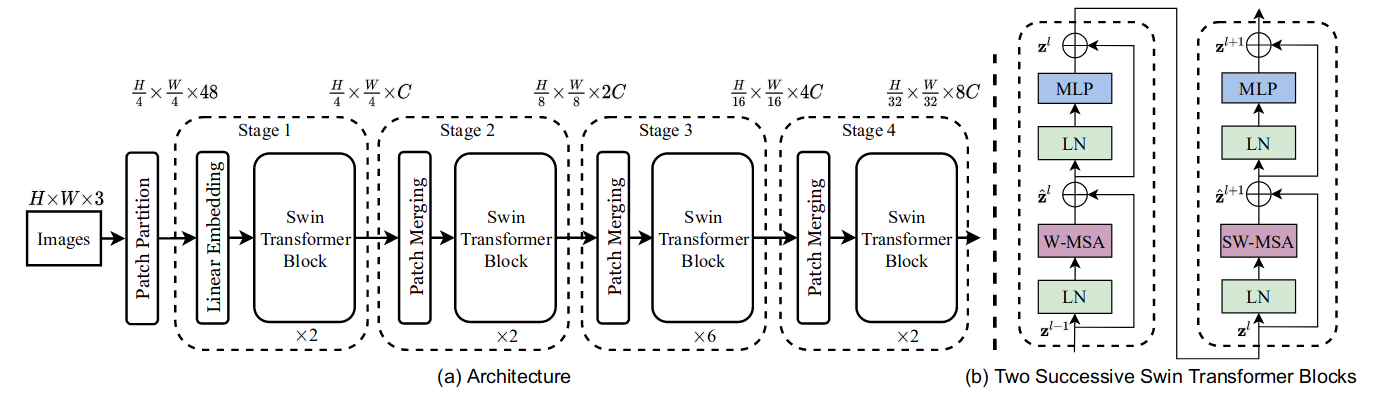
\includegraphics[width=\textwidth]{images/swin_architecture}}
	\caption{
	\textRL{بنية محول}
	\textLR{Swin-Tiny}
	\textLR{\cite{swintransformer}}}
	\label{fig:swin}
\end{figure}
\newline
يبين الشكل 
\ref{fig:swin}
 بنية المحول
\textLR{Swin-Tiny}،
وكما نلاحظ فإن الجزء الأول من المخطط هو
\textLR{patch partition}،
إذ يتم تقسيم الصورة إلى أجزاء 
\textLR{patches}
كما في خوارزمية
\textLR{ViT\cite{ViT}}،
%وهو كما يوضح الشكل
%\ref{fig:swin_patch_partition}،
%يتم بداية تقسيم الصورة إلى نوافذ وهي الخطوط الحمراء في الشكل، وكل نافذة تقسم إلى أجزاء
%\textLR{patches}
%وهي الخطوط الرمادية  كما في خوارزمية
%\textLR{\cite{ViT}}،
%\begin{figure}[!h]
%	\centerline{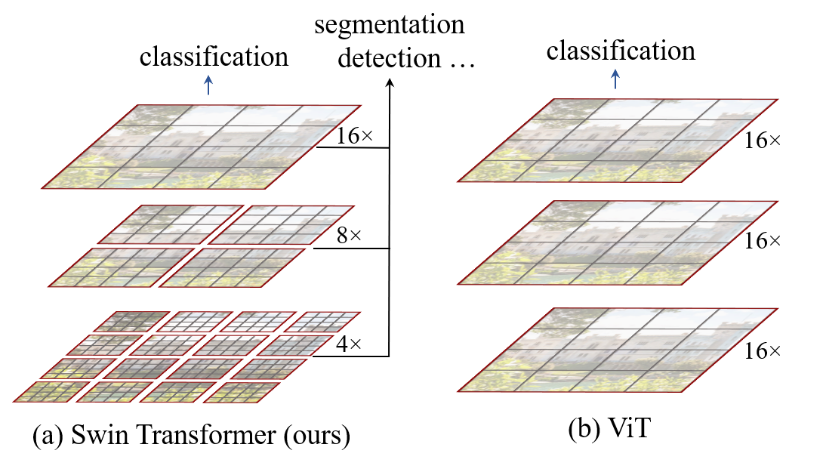
\includegraphics[width=\textwidth]{images/swin_patch_patition.png}}
%	\caption{
%	\textRL{الفرق بين تقسيم النوافذ بين محولي}
%	\textLR{ViT\cite{ViT},Swin\cite{swintransformer}}}
%	\label{fig:swin_patch_partition}
%\end{figure}
حيث يعامل كل جزء معاملة
\textLR{token}،
حجم كل جزء
$4\mathsf{x}4\mathsf{x}3 = 48$،
وبالتالي عدد عناصر سلسلة الدخل أو عدد الـ
\textLR{tokens}
هو
$(\frac{H}{4} \mathsf{x} \frac{W}{4})$.
فيكون دخل المرحلة الأولى
\textLR{stage1}
هو سلسلة بأبعاد
$\frac{HW}{16} \mathsf{x}48$.
\newline
الكتلة الأولى في المرحلة الأولى هي 
\textLR{linear embedding}،
وهي عبارة عن طبقة خطية هدفها إسقاط شعاع السمات السابق إلى بعد 
$C$
أي يصبح
$\frac{HW}{16}\mathsf{x}C$.
ومن ثم يتم تطبيق كتلتي محول 
\textLR{Swin}
متعاقبتين،  بنية الكتلة موضحة في الجزء اليمين من الشكل
\ref{fig:swin}
وسنشرحها في الفقرة القادمة، أبعاد دخل وخرج كتلة محول 
\textLR{Swin}
تبقى ثابتة، أي يكون بعد خرج المرحلة الأولى هو
$\frac{HW}{16}\mathsf{x}C$.
\subsubsection{الهرمية
\textLR{hierarchical}}
نلاحظ بأن الجزء الأول من كل مرحلة تالية هو طبقة
\textLR{patch merging}،
وهو القسم المسؤول عن هرمية النموذج، إذ أن هدف هذه الطبقة الخطية هو تخفيض عدد عناصر سلسلة الدخل أو الـ
\textLR{tokens}،
ويزداد هذا التخفيض  بازدياد عمق النموذج
 كما نلاحظ من أبعاد دخل كل كتلة في الشكل 
\ref{fig:swin}.
\newline
تقوم هذه الطبقة بدمج كل مجموعة
$2\mathsf{x}2$ 
من العناصر المتجاورة وتقوم بسلسلتها فتصبح شعاع واحد بـ$4$ عناصر، وبالتالي يتغير عدد عناصر السلسلة 
فإذا كانت أبعاد السلسلة
$\frac{H}{4}\mathsf{x}\frac{W}{4}\mathsf{x}C$ 
فيصبح
$\frac{H}{8}\mathsf{x}\frac{W}{8}\mathsf{x}4C$،
ومن ثم عبر طبقة خطية تقوم بتغيير أبعاد كل عنصر من السلسلة أو كل 
\textLR{token}
إلى النصف فيصبح
$\frac{H}{8}\mathsf{x}\frac{W}{8}\mathsf{x}2C$،
وهو خرج المرحلة الثانية.
\newline
$\frac{H}{16}\mathsf{x}\frac{W}{16}\mathsf{x}4C$ 
خرج المرحلة الثالثة.
\newline
$\frac{H}{32}\mathsf{x}\frac{W}{32}\mathsf{x}8C$
وهو خرج المرحلة الرابعة والأخيرة في نموذج
\textLR{tiny}.
\newline
إن أبعاد كل مرحلة مشابهة لأبعاد السمات في شبكات
\textLR{CNN}
النموذجية كما في
\textLR{VGG\cite{VGG}, ResNet\cite{ResNet}}
وهذا ما يمكننا من استخدام هذا النموذج كـ
\textLR{backbone}
بديل
لتطبيقات الرؤية الحاسوبية المختلفة.
\subsubsection{كتلة محول
\textLR{Swin}}
نلاحظ من الجزء اليسار من المخطط أن بنية 
\textLR{Swin}
مشابهة لبنية المحول الأصلي، فيما عدا استبدال الانتباه المتعدد الرؤوس 
\textLR{MHA}
بـ انتباه متعدد الرؤوس مع نوافذ
\textLR{W-MHA}
في الكتلة الأولى، وانتباه متعدد الرؤوس مع نوافذ مزاحة 
\textLR{SW-MHA}
في الكتلة التالية.
\subsubsection{التعقيد الحسابي عند استخدام النوافذ}
يوضح الشكل
\ref{fig:swin_shifted_window}
تقسيم النوافذ،
إذ يتم حساب الانتباه الذاتي بين عناصر النافذة الواحدة فقط، وهذا ما يخفض التعقيد الحسابي.
مقارنة بالمحول الأصلي الذي يحسب الانتباه الذاتي بين كل العناصر فإن التعقيد الحسابي من أجل سلسلة دخل بأبعاد 
$hw\mathsf{x}C$ 
يكون: 
\begin{equation}
\Omega(MHA) = 4hwC^2+2(hw)^2C
\end{equation}
نلاحظ أن التعقيد يزداد بشكل تربيعي مع زيادة أبعاد الصورة
بينما في حال استخدام طريقة النوافذ وحساب الانتباه داخل العناصر ضمن النافذة الواحدة فقط فيكون التعقيد الحسابي من أجل كل نافذة تحوي 
$M\mathsf{x}M$ 
جزء أو 
\textLR{patch}
يكون
\begin{equation}
\Omega(W-MHA)=4hwC^2+2M^2hwC
\end{equation}
نلاحظ بأن التعقيد الحسابي متناسب بشكل خطي مع أبعاد الصورة في حال كانت
$M$ 
ثابتة ( في النموذج 
$M=7$
)،
هذا التخفيض في التعقيد الحسابي يجعل من محول 
\textLR{Swin}
مناسب أكثر لتطبيقات الصورة ذات الحجوم الكبيرة و لتطبيقات الزمن الحقيقي.
\subsubsection{النوافذ المزاحة}
\begin{figure}[!h]
	\centerline{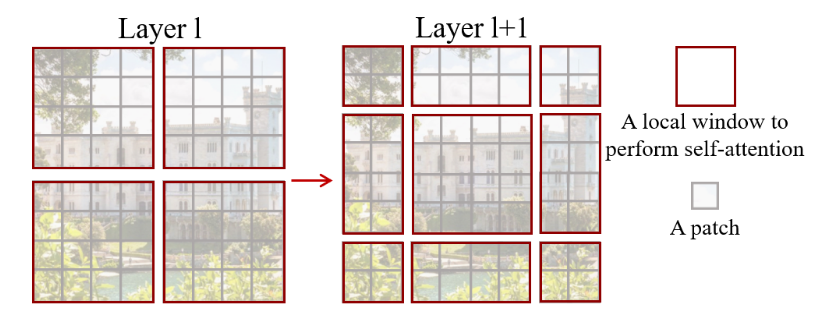
\includegraphics[width=\textwidth]{images/swin_shifted_window.png}}
	\caption{
	\textRL{طريقة النوافذ المزاحة بين كل كتلتين متعاقبتين في محول}
	\textLR{Swin}
	\textLR{\cite{swintransformer}}}
	\label{fig:swin_shifted_window}
\end{figure}
يبين الشكل
\ref{fig:swin_shifted_window}
كيفية اختيار تقسيم النوافذ من أجل كتلتين أو طبقتين متتاليتين من محول 
\textLR{Swin}.
الطبقة الأولى 
$l$
( الصورة اليسار) تقسم النوافذ بشكل نظامي، ويحسب الانتباه الذاتي ضمن أقسام النافذة الواحدة، كل نافذة على حدة.
الطبقة التالية من محول 
\textLR{Swin}
تقسم النوافذ بشكل مزاح عن نوافذ الطبقة السابقة، وذلك بمقدار نصف نافذة إلى جهة اليمين ونصف نافذة إلى الأسفل.
توضح المعادلات 
\ref{eq:swin_SW}
 خرج السمات من أجل كتلتين متعاقبتين لمحول 
\textLR{Swin} 
في مرحلة واحدة.
المعادلة الأولى تحسب الانتباه من أجل تقسيم النوافذ النظامي، الشكل
\ref{fig:swin_shifted_window}
 اليسار.
أما المعادلة الثالثة فهي حساب الانتباه ضمن النوافذ المزاحة، الشكل
\ref{fig:swin_shifted_window}
اليمين
\begin{equation}
	\begin{split}
	&\hat{z}^l = W-MSA(LN(z^{l-1}))+z^{l-1}\\
	&z^l = MLP(LN(\hat{z}^l))+\hat{z}^l\\
	&\hat{z}^{l+1} = SW-MSA(LN(z^l))+z^l\\
	&z^{l+1} = MLP(LN(\hat{z}^{l+1}))+\hat{z}^{l+1}\\
	\end{split}
	\label{eq:swin_SW}
\end{equation}
حيث 
$z_{l-1}$
خرج كتلة محول 
\textLR{Swin}
للمرحلة السابقة.
\subsubsection{تأثير النوافذ المزاحة وفائدتها}
نلاحظ أن النوافذ المزاحة في الطبقة 
$l+1$
تتقاطع مع نوافذ الطبقة 
$l$
ذات التقسيم النظامي، وهذا التقاطع يؤمن اتصال وتبادل معلومات بين النوافذ المجاورة كون الانتباه يحسب ضمن النافذة فقط، ويتجاهل النوافذ الأخرى.
طريقة النوافذ المزاحة قد حسنت من قدرة النمذجة للنموذج وهذا مايوضحه البحث 
\textLR{\cite{swintransformer}}
\subsubsection{الإزاحة الحلقية
\textLR{cyclic-shifting}}
ينتج عن طريقة النوافذ المزاحة زيادة في عدد النوافذ، بحيث لو كان عدد النوافذ في التقسيم النظامي
$\frac{h}{M} \mathsf{x} \frac{w}{M}$
يصبح في طبقة النوافذ المزاحة
$(\frac{h}{M} +1) \mathsf{x} (\frac{w}{M}+1)$،
حيث
$M \mathsf{x} M$
عدد أجزاء النافذة الواحدة. وكما في الشكل 
\ref{fig:swin_shifted_cycled_window}
 فإن بعض النوافذ سيكون حجمها أقل من 
$M\mathsf{x}M$.
أبسط طريقة لحل هذه المشكلة هي بحشو 
\textLR{pad}
النوافذ صغير الحجم لتصبح ببعد 
$M\mathsf{x}M$،
ومن ثم حساب الانتباه الذاتي داخل هذه النافذ  مع حجب القيم المحشوة.
هذا الحل لا يزيد من التعقيد الحسابي للنموذج حين يكون عدد النوافذ صغير، ولكن في حال العدد الكبير للنوافذ فقد اقترح النموذج طريقة الإزاحة الحلقية. 
\begin{figure}[!h]
	\centerline{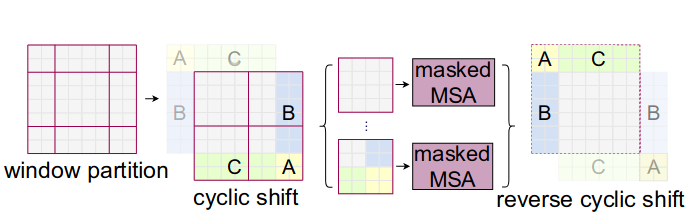
\includegraphics[width=\textwidth]{images/swin_shifted_cycled_window.png}}
	\caption{
		الازاحة الحلقية المستخدمة في محول
		\textLR{Swin}
		\textLR{\cite{swintransformer}}}
	\label{fig:swin_shifted_cycled_window}
\end{figure}
هذه الطريقة كما يوضح الشكل 
\ref{fig:swin_shifted_cycled_window}
 فإنه يتم إعادة ترتيب الأقسام بشكل حلقي حتى يكون عدد النوافذ متساوِ قبل وبعد الإزاحة. وأثناء إعادة الترتيب بشكل حلقي يمكن أن تحتوي النافذة على أجزاء من النوافذ الأخرى غير المجاورة لها،  ولحساب الانتباه الذاتي في هذه الحالة نستخدم تقنية الحجب 
\textLR{masking}
 وذلك لكي لا تدخل النوافذ غير المجاورة في حساب الانتباه الذاتي.
في هذه الحالة نحافظ على عدد النوافذ في حال التقسيم النظامي وفي حال التقسيم المزاح.
بينت التجربة في المقالة
\textLR{\cite{swintransformer}}
أن طريقة الازاحة الحلقية أسرع من طريق الحشو.
\begin{figure}[!h]
	\centerline{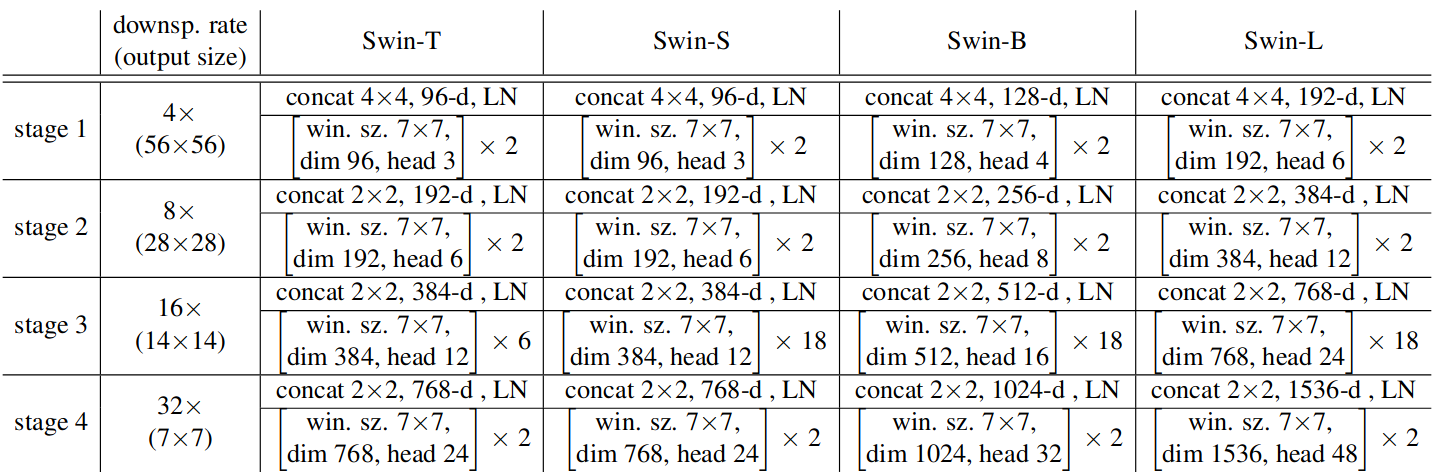
\includegraphics[width=\textwidth]{images/swin_architecture_table.png}}
	\caption{
	\textRL{أبعاد نموذج }
	\textLR{Swin}
	\textRL{من أجل عدة نسخ}
	\textLR{\cite{swintransformer}}}
	\label{fig:swin_architecture_table}
\end{figure}
يبين الجدول 
\ref{fig:swin_architecture_table}
أبعاد كل مرحلة من مراحل محول 
\textLR{Swin}
وذلك من أجل أبعاد مختلفة لصورة الدخل (السطر الأول من الجدول)، من أجل ملاحق
\textLR{Swin} 
فقد تم تدريبه من أجل عدة نسخ من المحول، اخترنا تطوير النسخة التي تستخدم
\textLR{Swin-Tiny}
كونه النموذج الأسرع والأقل كلفة في التدريب.